\documentclass[tikz,margin=3pt]{standalone}
% \documentclass{article}
\pagestyle{empty}
\usepackage{tikz}
\usepackage{pgfplots}
\usetikzlibrary{calc}
\usetikzlibrary{shapes.geometric}
\usetikzlibrary{shapes.misc, positioning}


\newcommand{\radius}{0.5}
\newcommand{\relposX}{1.5}
\newcommand{\relposY}{-1.5}
\newcommand{\circX}{-1}
\newcommand{\circY}{0}
\newcommand{\shiftY}{0}

\begin{document}



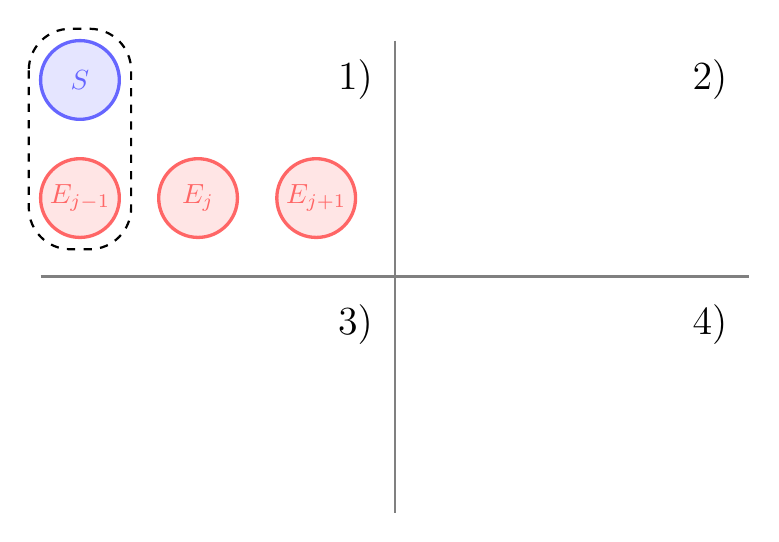
\begin{tikzpicture}
\draw[gray, very thick] (-1.5,-2.5) -- (7.5,-2.5);
\draw[gray, thick] (3,0.5) -- (3, -5.5);
\node at (2.5,0) (S2) {\Large{1)}};
\node at (7,0) (S2) {\Large{2)}};
\node at (2.5,-3.1) (S2) {\Large{3)}};
\node at (7,-3.1) (S2) {\Large{4)}};

\begin{scope}[shift={(0,0)}]
    \filldraw[color=blue!60, fill=blue!10, very thick](\circX,\circY) circle (\radius) node {\(S\)};
    \filldraw[color=red!60, fill=red!10, very thick](\circX,\relposY) circle (\radius) node {\(E_{j-1}\)};
    \filldraw[color=red!60, fill=red!10, very thick](\circX+\relposX,\relposY) circle (\radius) node {\(E_{j}\)};
    \filldraw[color=red!60, fill=red!10, very thick](\circX+2*\relposX,\relposY) circle (\radius) node {\(E_{j+1}\)};
    \draw[rounded corners=15, dashed, thick] (\circX-1.3*\radius, \circY+1.3*\radius) rectangle (-\radius + 0.15, \relposY-\radius-0.15) {};
\end{scope}


\end{tikzpicture}


\end{document}

% \begin{scope}[shift={(5,-3.5)}]
%     \filldraw[color=blue!60, fill=blue!10, very thick](\circX+\relposX,\circY) circle (\radius) node {\(S\)};
%     \filldraw[color=red!60, fill=red!10, very thick](-1,\relposY) circle (\radius) node {\(E_{j-1}\)};
%     \filldraw[color=red!60, fill=red!10, very thick](\circX+\relposX,\relposY) circle (\radius) node {\(E_{j}\)};
%     \filldraw[color=red!60, fill=red!10, very thick](\circX+2*\relposX,\relposY) circle (\radius) node {\(E_{j+1}\)};
%     \draw[rounded corners=15, dashed] (\circX-1.3*\radius+\relposX, \circY+1.3*\radius) rectangle (-\radius + 0.15 +\relposX, \relposY-\radius-0.15) {};
%     \draw[rounded corners=15, dashed, thick] (\circX-1.3*\radius + \relposX, \circY+\relposY+\radius+0.15) rectangle (\circX+2*\relposX+\radius+0.15, \relposY-\radius-0.15) {};
% \end{scope}